\documentclass[a4paper]{book}
\usepackage{makeidx}
\usepackage{graphicx}
\usepackage{multicol}
\usepackage{float}
\usepackage{listings}
\usepackage{color}
\usepackage{ifthen}
\usepackage[table]{xcolor}
\usepackage{textcomp}
\usepackage{alltt}
\usepackage{ifpdf}
\ifpdf
\usepackage[pdftex,
            pagebackref=true,
            colorlinks=true,
            linkcolor=blue,
            unicode
           ]{hyperref}
\else
\usepackage[ps2pdf,
            pagebackref=true,
            colorlinks=true,
            linkcolor=blue,
            unicode
           ]{hyperref}
\usepackage{pspicture}
\fi
\usepackage[utf8]{inputenc}
\usepackage{mathptmx}
\usepackage[scaled=.90]{helvet}
\usepackage{courier}
\usepackage{sectsty}
\usepackage[titles]{tocloft}
\usepackage{doxygen}
\lstset{language=C++,inputencoding=utf8,basicstyle=\footnotesize,breaklines=true,breakatwhitespace=true,tabsize=8,numbers=left }
\makeindex
\setcounter{tocdepth}{3}
\renewcommand{\footrulewidth}{0.4pt}
\renewcommand{\familydefault}{\sfdefault}
\begin{document}
\hypersetup{pageanchor=false}
\begin{titlepage}
\vspace*{7cm}
\begin{center}
{\Large WIA Battlezone \\[1ex]\large 1.0 }\\
\vspace*{1cm}
{\large Generated by Doxygen 1.7.4}\\
\vspace*{0.5cm}
{\small Sat Apr 16 2011 17:45:45}\\
\end{center}
\end{titlepage}
\clearemptydoublepage
\pagenumbering{roman}
\tableofcontents
\clearemptydoublepage
\pagenumbering{arabic}
\hypersetup{pageanchor=true}
\chapter{Class Index}
\section{Class Hierarchy}
This inheritance list is sorted roughly, but not completely, alphabetically:\begin{DoxyCompactList}
\item \contentsline{section}{CS325Graphics}{\pageref{class_c_s325_graphics}}{}
\item \contentsline{section}{Object}{\pageref{class_object}}{}
\item \contentsline{section}{Point}{\pageref{class_point}}{}
\begin{DoxyCompactList}
\item \contentsline{section}{Pose}{\pageref{class_pose}}{}
\end{DoxyCompactList}
\item \contentsline{section}{Point2D}{\pageref{class_point2_d}}{}
\item \contentsline{section}{Point3D}{\pageref{class_point3_d}}{}
\item \contentsline{section}{Vector2D}{\pageref{class_vector2_d}}{}
\item \contentsline{section}{Vector3D}{\pageref{class_vector3_d}}{}
\end{DoxyCompactList}

\chapter{Class Index}
\section{Class List}
Here are the classes, structs, unions and interfaces with brief descriptions:\begin{DoxyCompactList}
\item\contentsline{section}{\hyperlink{class_c_s325_graphics}{CS325Graphics} }{\pageref{class_c_s325_graphics}}{}
\item\contentsline{section}{\hyperlink{class_point}{Point} (This class is used to store x,y, and z coordinates )}{\pageref{class_point}}{}
\item\contentsline{section}{\hyperlink{class_point2_d}{Point2D} }{\pageref{class_point2_d}}{}
\item\contentsline{section}{\hyperlink{class_point3_d}{Point3D} }{\pageref{class_point3_d}}{}
\item\contentsline{section}{\hyperlink{class_pose}{Pose} (This class is used to store a position and is a subclass of \hyperlink{_point_8h_source}{Point.h} )}{\pageref{class_pose}}{}
\item\contentsline{section}{\hyperlink{class_vector2_d}{Vector2D} }{\pageref{class_vector2_d}}{}
\item\contentsline{section}{\hyperlink{class_vector3_d}{Vector3D} }{\pageref{class_vector3_d}}{}
\end{DoxyCompactList}

\chapter{Class Documentation}
\hypertarget{class_c_s325_graphics}{
\section{CS325Graphics Class Reference}
\label{class_c_s325_graphics}\index{CS325Graphics@{CS325Graphics}}
}
\subsection*{Public Member Functions}
\begin{DoxyCompactItemize}
\item 
\hypertarget{class_c_s325_graphics_a6f85502405f075faafae55dbe3271524}{
{\bfseries CS325Graphics} (int, char $\ast$\mbox{[}$\,$\mbox{]})}
\label{class_c_s325_graphics_a6f85502405f075faafae55dbe3271524}

\item 
\hypertarget{class_c_s325_graphics_a50bef85ed0e65160e4035f8333737269}{
void {\bfseries DrawLineOnScreen} (\hyperlink{class_point2_d}{Point2D} p1, \hyperlink{class_point2_d}{Point2D} p2)}
\label{class_c_s325_graphics_a50bef85ed0e65160e4035f8333737269}

\item 
\hypertarget{class_c_s325_graphics_a6d50fae71655d3ae1447a5cab911057a}{
void {\bfseries DrawLineInSpace} (\hyperlink{class_point3_d}{Point3D} p1, \hyperlink{class_point3_d}{Point3D} p2)}
\label{class_c_s325_graphics_a6d50fae71655d3ae1447a5cab911057a}

\item 
\hypertarget{class_c_s325_graphics_a6e675e1c68c76bd09fcb4437057a2ca6}{
void {\bfseries DisplayNow} ()}
\label{class_c_s325_graphics_a6e675e1c68c76bd09fcb4437057a2ca6}

\item 
\hypertarget{class_c_s325_graphics_a87ce4123a68fb75d29e72dd236f5aab7}{
void {\bfseries SetViewPosition} (\hyperlink{class_point2_d}{Point2D} vp)}
\label{class_c_s325_graphics_a87ce4123a68fb75d29e72dd236f5aab7}

\item 
\hypertarget{class_c_s325_graphics_a317b9241e6bee5575b5d2914b40f6de3}{
void {\bfseries SetViewDirection} (\hyperlink{class_vector2_d}{Vector2D} vd)}
\label{class_c_s325_graphics_a317b9241e6bee5575b5d2914b40f6de3}

\end{DoxyCompactItemize}
\subsection*{Static Public Attributes}
\begin{DoxyCompactItemize}
\item 
\hypertarget{class_c_s325_graphics_ad36a4f7cb61ffc2cc6c66da132d63c25}{
static const float {\bfseries X\_\-MAX}}
\label{class_c_s325_graphics_ad36a4f7cb61ffc2cc6c66da132d63c25}

\item 
\hypertarget{class_c_s325_graphics_a4b011e0ec3b09eb067473d8eeb0fda94}{
static const float {\bfseries Y\_\-MAX}}
\label{class_c_s325_graphics_a4b011e0ec3b09eb067473d8eeb0fda94}

\item 
\hypertarget{class_c_s325_graphics_a9b11863e11d057be42bd107ab557360d}{
static const float {\bfseries X\_\-MIN}}
\label{class_c_s325_graphics_a9b11863e11d057be42bd107ab557360d}

\item 
\hypertarget{class_c_s325_graphics_a42ea775ab5872ae0129569f596afda92}{
static const float {\bfseries Y\_\-MIN}}
\label{class_c_s325_graphics_a42ea775ab5872ae0129569f596afda92}

\end{DoxyCompactItemize}


The documentation for this class was generated from the following file:\begin{DoxyCompactItemize}
\item 
U:/battlezone/WIA\_\-Battlezone/WIA\_\-Battlezone/cs325graphics.h\end{DoxyCompactItemize}

\hypertarget{class_point}{
\section{Point Class Reference}
\label{class_point}\index{Point@{Point}}
}


{\ttfamily \#include $<$Point.h$>$}

Inheritance diagram for Point:\begin{figure}[H]
\begin{center}
\leavevmode
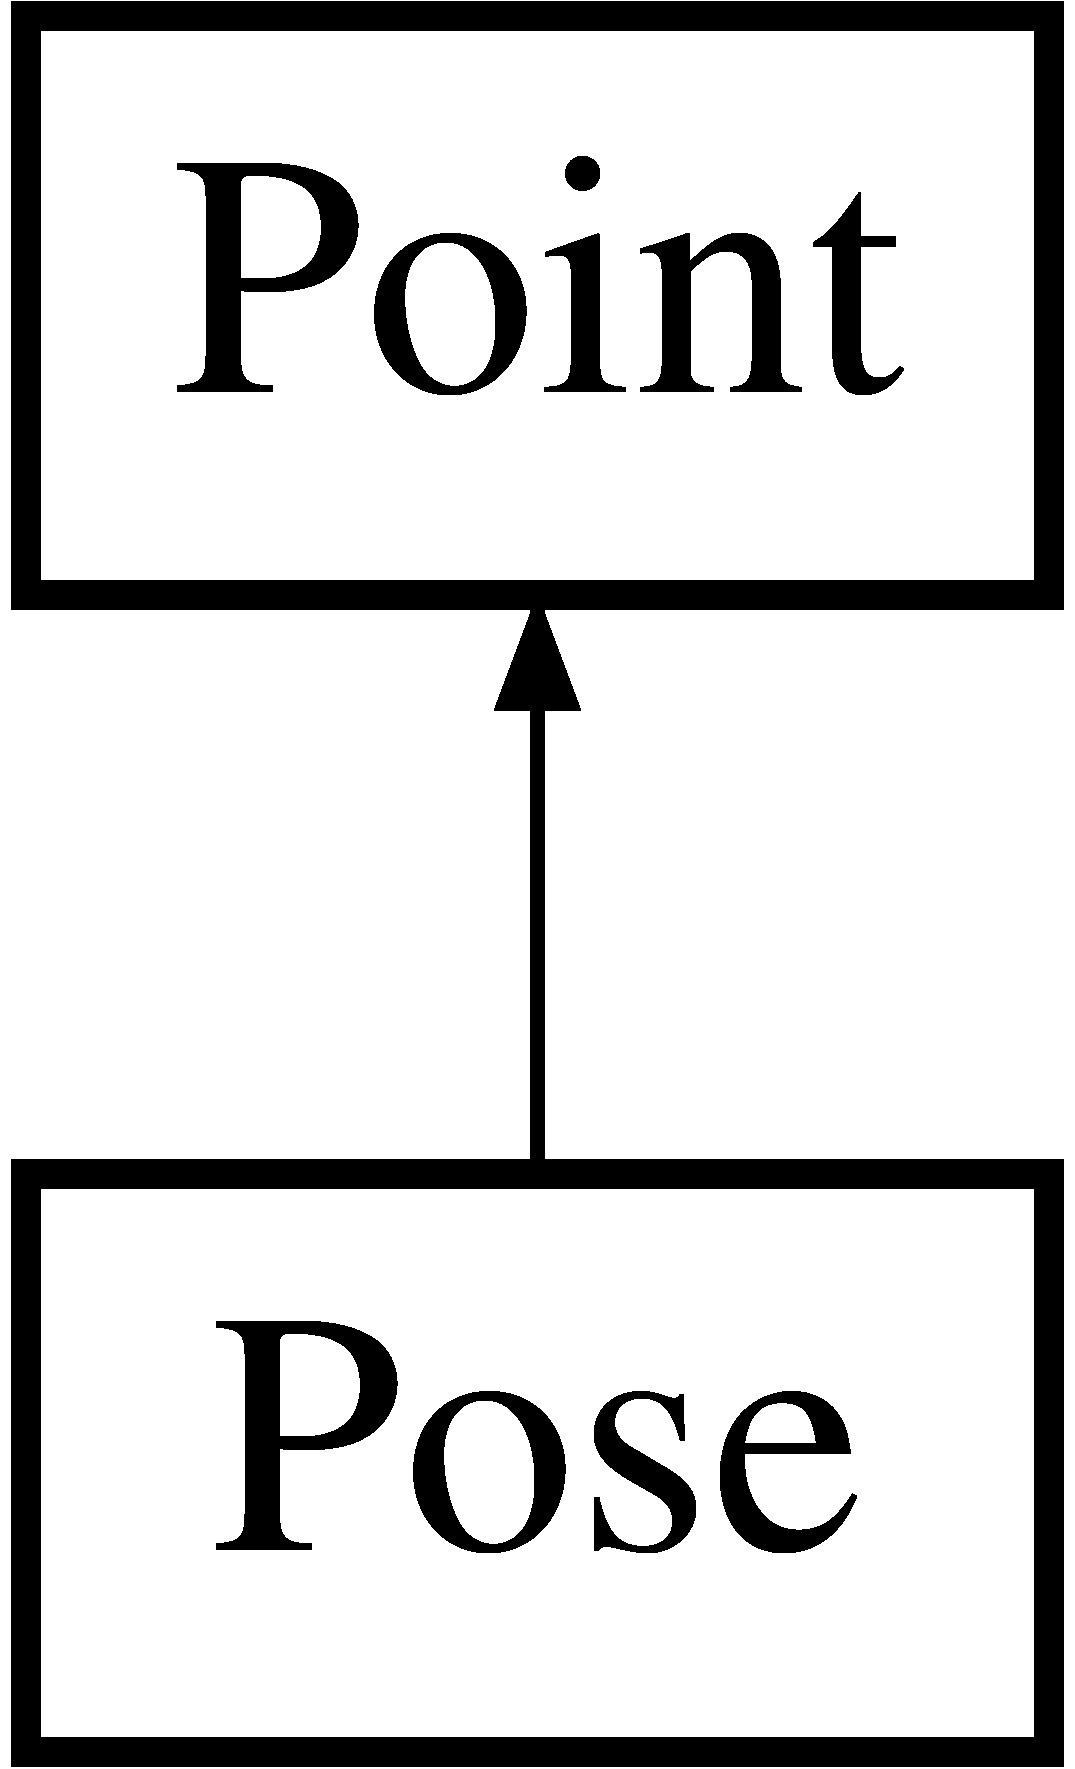
\includegraphics[height=2.000000cm]{class_point}
\end{center}
\end{figure}
\subsection*{Public Member Functions}
\begin{DoxyCompactItemize}
\item 
\hyperlink{class_point_ad92f2337b839a94ce97dcdb439b4325a}{Point} ()
\item 
\hyperlink{class_point_aef2feff94db53418730e802319eb4fe7}{Point} (float \_\-x, float \_\-y, float \_\-z)
\item 
float \hyperlink{class_point_acc27466778cc87a662bba40268c4c0c8}{getX} ()
\item 
float \hyperlink{class_point_a3cccbca94719ddde353cce86ce0e2f64}{getY} ()
\item 
float \hyperlink{class_point_adfd464bbfabdcecdcc14eb83cf6d2830}{getZ} ()
\item 
void \hyperlink{class_point_af2a602d5d53872fff27313639da37e3b}{setPoint} (float \_\-x, float \_\-y, float \_\-z)
\item 
void \hyperlink{class_point_ac2ef23aa700771edccd87a19b82104c9}{setPoint} (\hyperlink{class_point}{Point} \_\-point)
\end{DoxyCompactItemize}


\subsection{Detailed Description}
A class that is used to store X, Y, and Z float values used as coordinates \begin{DoxyAuthor}{Author}
Ben Hubler 
\end{DoxyAuthor}
\begin{DoxyDate}{Date}
4/14/2011 
\end{DoxyDate}
\begin{DoxyVersion}{Version}
1.0 
\end{DoxyVersion}


\subsection{Constructor \& Destructor Documentation}
\hypertarget{class_point_ad92f2337b839a94ce97dcdb439b4325a}{
\index{Point@{Point}!Point@{Point}}
\index{Point@{Point}!Point@{Point}}
\subsubsection[{Point}]{\setlength{\rightskip}{0pt plus 5cm}Point::Point (
\begin{DoxyParamCaption}
{}
\end{DoxyParamCaption}
)}}
\label{class_point_ad92f2337b839a94ce97dcdb439b4325a}
Default constructor sets default values for x,y, and z to 0.0 during initialization \hypertarget{class_point_aef2feff94db53418730e802319eb4fe7}{
\index{Point@{Point}!Point@{Point}}
\index{Point@{Point}!Point@{Point}}
\subsubsection[{Point}]{\setlength{\rightskip}{0pt plus 5cm}Point::Point (
\begin{DoxyParamCaption}
\item[{float}]{\_\-x, }
\item[{float}]{\_\-y, }
\item[{float}]{\_\-z}
\end{DoxyParamCaption}
)}}
\label{class_point_aef2feff94db53418730e802319eb4fe7}
Overloaded constructor to set x,y, and z during initialization 
\begin{DoxyParams}{Parameters}
{\em \_\-x} & is a float representing the X coordinate \\
\hline
{\em \_\-y} & is a float representing the Y coordinate \\
\hline
{\em \_\-z} & is a float representing the Z coordinate \\
\hline
\end{DoxyParams}


\subsection{Member Function Documentation}
\hypertarget{class_point_acc27466778cc87a662bba40268c4c0c8}{
\index{Point@{Point}!getX@{getX}}
\index{getX@{getX}!Point@{Point}}
\subsubsection[{getX}]{\setlength{\rightskip}{0pt plus 5cm}float Point::getX (
\begin{DoxyParamCaption}
{}
\end{DoxyParamCaption}
)}}
\label{class_point_acc27466778cc87a662bba40268c4c0c8}
Function to return X coordinate \begin{DoxyReturn}{Returns}
a float representing the X coordinate 
\end{DoxyReturn}
\hypertarget{class_point_a3cccbca94719ddde353cce86ce0e2f64}{
\index{Point@{Point}!getY@{getY}}
\index{getY@{getY}!Point@{Point}}
\subsubsection[{getY}]{\setlength{\rightskip}{0pt plus 5cm}float Point::getY (
\begin{DoxyParamCaption}
{}
\end{DoxyParamCaption}
)}}
\label{class_point_a3cccbca94719ddde353cce86ce0e2f64}
Function to return Y coordinate \begin{DoxyReturn}{Returns}
a float representing the Y coordinate 
\end{DoxyReturn}
\hypertarget{class_point_adfd464bbfabdcecdcc14eb83cf6d2830}{
\index{Point@{Point}!getZ@{getZ}}
\index{getZ@{getZ}!Point@{Point}}
\subsubsection[{getZ}]{\setlength{\rightskip}{0pt plus 5cm}float Point::getZ (
\begin{DoxyParamCaption}
{}
\end{DoxyParamCaption}
)}}
\label{class_point_adfd464bbfabdcecdcc14eb83cf6d2830}
Function to return Z coordinate \begin{DoxyReturn}{Returns}
a float representing the Z coordinate 
\end{DoxyReturn}
\hypertarget{class_point_af2a602d5d53872fff27313639da37e3b}{
\index{Point@{Point}!setPoint@{setPoint}}
\index{setPoint@{setPoint}!Point@{Point}}
\subsubsection[{setPoint}]{\setlength{\rightskip}{0pt plus 5cm}void Point::setPoint (
\begin{DoxyParamCaption}
\item[{float}]{\_\-x, }
\item[{float}]{\_\-y, }
\item[{float}]{\_\-z}
\end{DoxyParamCaption}
)}}
\label{class_point_af2a602d5d53872fff27313639da37e3b}
Function to set X,Y, and Z coordinates 
\begin{DoxyParams}{Parameters}
{\em \_\-x} & is a float representing the X coordinate \\
\hline
{\em \_\-y} & is a float representing the Y coordinate \\
\hline
{\em \_\-z} & is a float representing the Z coordinate \\
\hline
\end{DoxyParams}
\hypertarget{class_point_ac2ef23aa700771edccd87a19b82104c9}{
\index{Point@{Point}!setPoint@{setPoint}}
\index{setPoint@{setPoint}!Point@{Point}}
\subsubsection[{setPoint}]{\setlength{\rightskip}{0pt plus 5cm}void Point::setPoint (
\begin{DoxyParamCaption}
\item[{{\bf Point}}]{\_\-point}
\end{DoxyParamCaption}
)}}
\label{class_point_ac2ef23aa700771edccd87a19b82104c9}
Function to set X,Y, and Z coordinates 
\begin{DoxyParams}{Parameters}
{\em \_\-point} & is a \hyperlink{class_point}{Point} representing the X, Y, and Z coordinates \\
\hline
\end{DoxyParams}


The documentation for this class was generated from the following files:\begin{DoxyCompactItemize}
\item 
U:/battlezone/WIA\_\-Battlezone/WIA\_\-Battlezone/\hyperlink{_point_8h}{Point.h}\item 
U:/battlezone/WIA\_\-Battlezone/WIA\_\-Battlezone/\hyperlink{_point_8cpp}{Point.cpp}\end{DoxyCompactItemize}

\hypertarget{class_point2_d}{
\section{Point2D Class Reference}
\label{class_point2_d}\index{Point2D@{Point2D}}
}


{\ttfamily \#include $<$point2d.h$>$}

\subsection*{Public Member Functions}
\begin{DoxyCompactItemize}
\item 
\hyperlink{class_point2_d_a1b119032e0b60ef27f8610d640e241e2}{Point2D} (void)
\item 
\hypertarget{class_point2_d_aeee3d27d547e4e4eb565bc91c0ea38d4}{
{\bfseries Point2D} (const \hyperlink{class_point2_d}{Point2D} \&p)}
\label{class_point2_d_aeee3d27d547e4e4eb565bc91c0ea38d4}

\item 
\hypertarget{class_point2_d_a0262726e46d2f7c32e886d98ba6b72a1}{
{\bfseries Point2D} (float x, float y)}
\label{class_point2_d_a0262726e46d2f7c32e886d98ba6b72a1}

\item 
\hypertarget{class_point2_d_ae85945d6f3dd852fc7b54a62876ceec0}{
void {\bfseries setX} (float x)}
\label{class_point2_d_ae85945d6f3dd852fc7b54a62876ceec0}

\item 
\hypertarget{class_point2_d_a0f99b0f7576dbeefafd88c545d80e061}{
void {\bfseries setY} (float y)}
\label{class_point2_d_a0f99b0f7576dbeefafd88c545d80e061}

\item 
\hypertarget{class_point2_d_a8a76ed85865034ac6b89053bb0d3eefb}{
void {\bfseries setXY} (float x, float y)}
\label{class_point2_d_a8a76ed85865034ac6b89053bb0d3eefb}

\item 
\hypertarget{class_point2_d_a1d99db0ab55004e689f6df96fe159fb8}{
float {\bfseries getX} ()}
\label{class_point2_d_a1d99db0ab55004e689f6df96fe159fb8}

\item 
\hypertarget{class_point2_d_ae4a95e28df1efd23b68a377b35624cfd}{
float {\bfseries getY} ()}
\label{class_point2_d_ae4a95e28df1efd23b68a377b35624cfd}

\item 
\hypertarget{class_point2_d_af6db77bd62da9048a360e099ac36b569}{
string {\bfseries toString} ()}
\label{class_point2_d_af6db77bd62da9048a360e099ac36b569}

\item 
void \hyperlink{class_point2_d_a7f0d35c684e22b47fc42cb142ec6c50e}{setFromString} (string \&s)
\end{DoxyCompactItemize}


\subsection{Detailed Description}
this class is used in the graphics portion of the tank project 

\subsection{Constructor \& Destructor Documentation}
\hypertarget{class_point2_d_a1b119032e0b60ef27f8610d640e241e2}{
\index{Point2D@{Point2D}!Point2D@{Point2D}}
\index{Point2D@{Point2D}!Point2D@{Point2D}}
\subsubsection[{Point2D}]{\setlength{\rightskip}{0pt plus 5cm}Point2D::Point2D (
\begin{DoxyParamCaption}
\item[{void}]{}
\end{DoxyParamCaption}
)}}
\label{class_point2_d_a1b119032e0b60ef27f8610d640e241e2}
\href{file:}{\tt file:} Point2D.cpp version: 0.91 author: djb date 28Nov07 

\subsection{Member Function Documentation}
\hypertarget{class_point2_d_a7f0d35c684e22b47fc42cb142ec6c50e}{
\index{Point2D@{Point2D}!setFromString@{setFromString}}
\index{setFromString@{setFromString}!Point2D@{Point2D}}
\subsubsection[{setFromString}]{\setlength{\rightskip}{0pt plus 5cm}void Point2D::setFromString (
\begin{DoxyParamCaption}
\item[{string \&}]{s}
\end{DoxyParamCaption}
)}}
\label{class_point2_d_a7f0d35c684e22b47fc42cb142ec6c50e}
read the first part of a string to set the value, and modify the string removing the value read. 
\begin{DoxyParams}{Parameters}
{\em s} & -\/ the string to read \\
\hline
\end{DoxyParams}


The documentation for this class was generated from the following files:\begin{DoxyCompactItemize}
\item 
U:/battlezone/WIA\_\-Battlezone/WIA\_\-Battlezone/point2d.h\item 
U:/battlezone/WIA\_\-Battlezone/WIA\_\-Battlezone/point2d.cpp\end{DoxyCompactItemize}

\hypertarget{class_point3_d}{
\section{Point3D Class Reference}
\label{class_point3_d}\index{Point3D@{Point3D}}
}


{\ttfamily \#include $<$point3d.h$>$}

\subsection*{Public Member Functions}
\begin{DoxyCompactItemize}
\item 
\hyperlink{class_point3_d_a4e65cd9031f66ffe6ed55102d4007128}{Point3D} (void)
\item 
\hypertarget{class_point3_d_a6781161506cdaa4a1425a57cab9b10ec}{
{\bfseries Point3D} (const \hyperlink{class_point3_d}{Point3D} \&p)}
\label{class_point3_d_a6781161506cdaa4a1425a57cab9b10ec}

\item 
\hypertarget{class_point3_d_a9a9cbd36f7da8cf5d5ee26ae341c1d90}{
{\bfseries Point3D} (float x, float y, float z)}
\label{class_point3_d_a9a9cbd36f7da8cf5d5ee26ae341c1d90}

\item 
\hypertarget{class_point3_d_ab4eeac67f15d8c07d508d4fa76b010b2}{
void {\bfseries setX} (float x)}
\label{class_point3_d_ab4eeac67f15d8c07d508d4fa76b010b2}

\item 
\hypertarget{class_point3_d_ac86480c69b4a32574f1339cea148f52e}{
void {\bfseries setY} (float y)}
\label{class_point3_d_ac86480c69b4a32574f1339cea148f52e}

\item 
\hypertarget{class_point3_d_aaefb320d17d263355e784cc4ec5912a9}{
void {\bfseries setZ} (float z)}
\label{class_point3_d_aaefb320d17d263355e784cc4ec5912a9}

\item 
\hypertarget{class_point3_d_ae9cf13cf431876d6048ac692652e2f4b}{
void {\bfseries setXYZ} (float x, float y, float z)}
\label{class_point3_d_ae9cf13cf431876d6048ac692652e2f4b}

\item 
\hypertarget{class_point3_d_a7f0dd2ed896a8d081232e11ce6d0ab60}{
float {\bfseries getX} ()}
\label{class_point3_d_a7f0dd2ed896a8d081232e11ce6d0ab60}

\item 
\hypertarget{class_point3_d_a7282c6b4c314622d37424d19fddeef53}{
float {\bfseries getY} ()}
\label{class_point3_d_a7282c6b4c314622d37424d19fddeef53}

\item 
\hypertarget{class_point3_d_abe4d040aab071fe4d0b5d13c1421fbf0}{
float {\bfseries getZ} ()}
\label{class_point3_d_abe4d040aab071fe4d0b5d13c1421fbf0}

\item 
\hypertarget{class_point3_d_a563bf7157eee202ebafb4031033ea5b6}{
void {\bfseries translate} (\hyperlink{class_vector3_d}{Vector3D} vector)}
\label{class_point3_d_a563bf7157eee202ebafb4031033ea5b6}

\item 
\hypertarget{class_point3_d_ad135ec7452f88baf82d4e714a6130d65}{
string {\bfseries toString} ()}
\label{class_point3_d_ad135ec7452f88baf82d4e714a6130d65}

\end{DoxyCompactItemize}


\subsection{Detailed Description}
this class is used in the graphics portion of the tank project 

\subsection{Constructor \& Destructor Documentation}
\hypertarget{class_point3_d_a4e65cd9031f66ffe6ed55102d4007128}{
\index{Point3D@{Point3D}!Point3D@{Point3D}}
\index{Point3D@{Point3D}!Point3D@{Point3D}}
\subsubsection[{Point3D}]{\setlength{\rightskip}{0pt plus 5cm}Point3D::Point3D (
\begin{DoxyParamCaption}
\item[{void}]{}
\end{DoxyParamCaption}
)}}
\label{class_point3_d_a4e65cd9031f66ffe6ed55102d4007128}
\href{file:}{\tt file:} point3D.cpp version: 1.0 author: djb date 12 April 2011 

The documentation for this class was generated from the following files:\begin{DoxyCompactItemize}
\item 
U:/battlezone/WIA\_\-Battlezone/WIA\_\-Battlezone/point3d.h\item 
U:/battlezone/WIA\_\-Battlezone/WIA\_\-Battlezone/point3d.cpp\end{DoxyCompactItemize}

\hypertarget{class_pose}{
\section{Pose Class Reference}
\label{class_pose}\index{Pose@{Pose}}
}


This class is used to store a position and is a subclass of \hyperlink{_point_8h_source}{Point.h}.  




{\ttfamily \#include $<$Pose.h$>$}

Inheritance diagram for Pose:\begin{figure}[H]
\begin{center}
\leavevmode
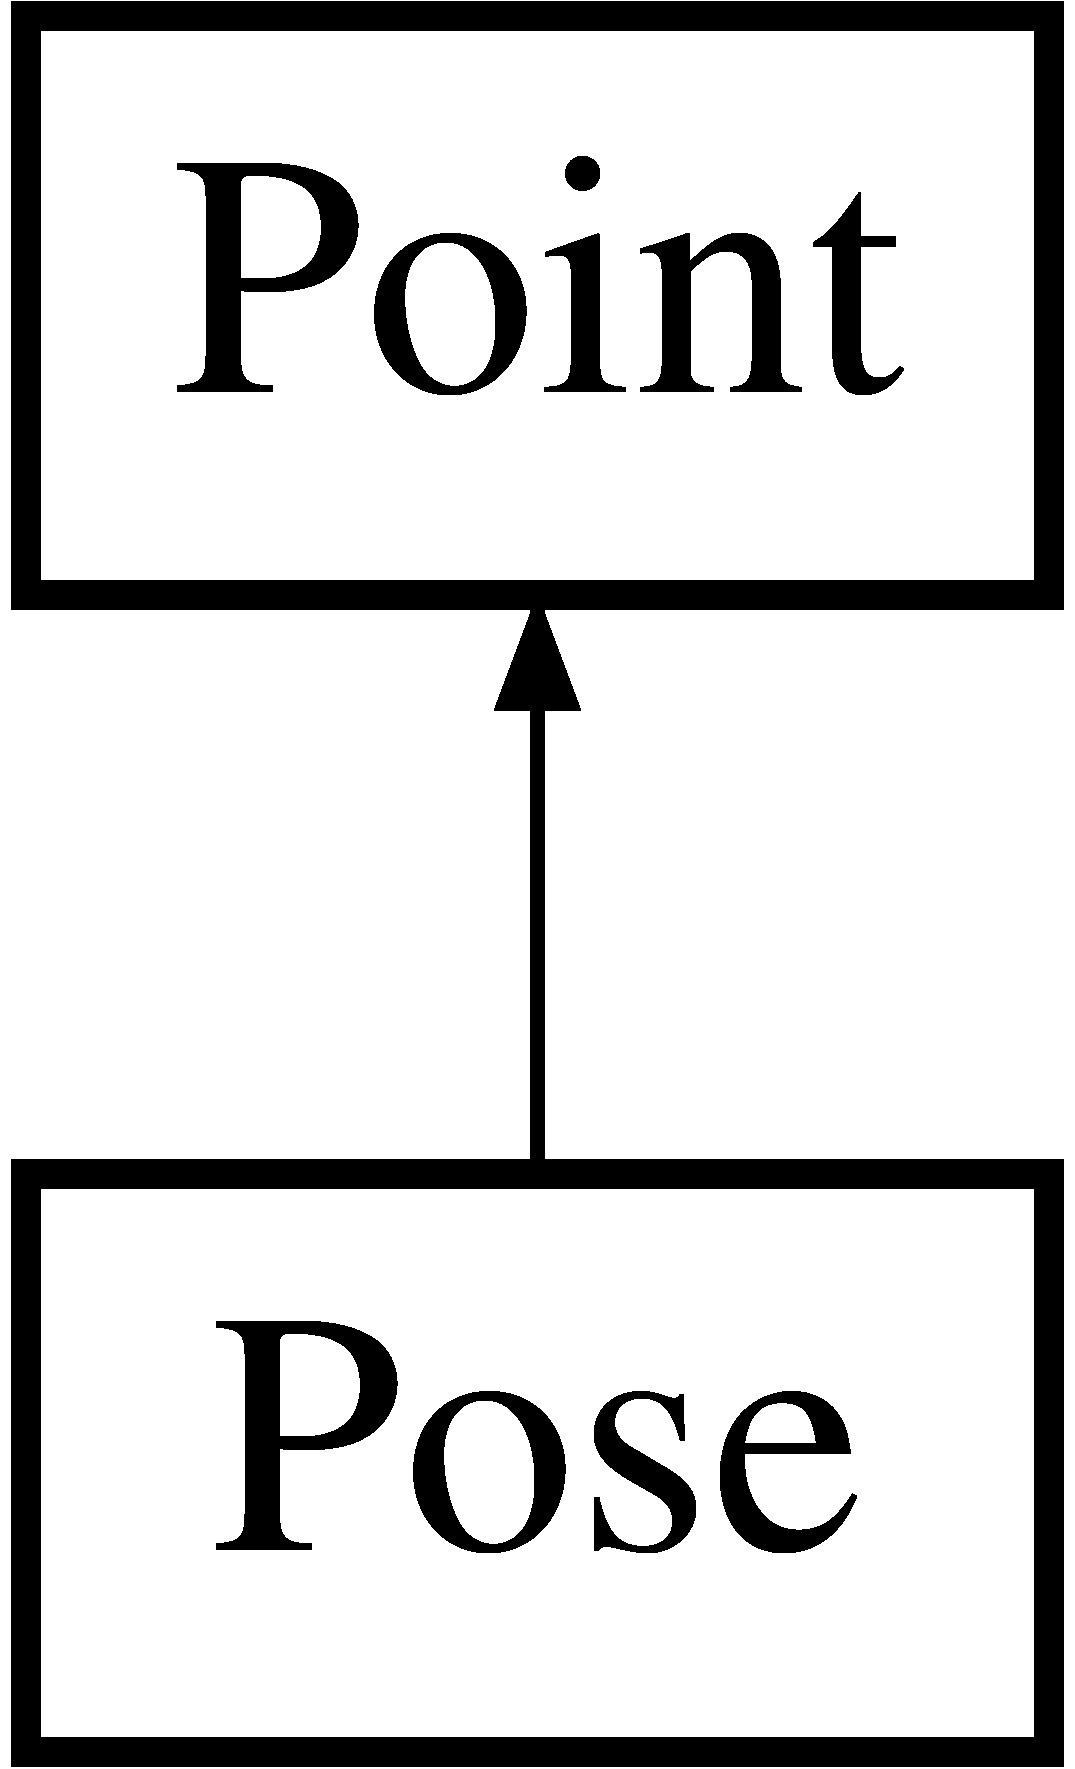
\includegraphics[height=2.000000cm]{class_pose}
\end{center}
\end{figure}
\subsection*{Public Member Functions}
\begin{DoxyCompactItemize}
\item 
\hypertarget{class_pose_a3cd8aa60acd61ec0d1ea7cf2da0f1bc7}{
{\bfseries Pose} (float \_\-x, float \_\-y, float \_\-z, float \_\-theta)}
\label{class_pose_a3cd8aa60acd61ec0d1ea7cf2da0f1bc7}

\item 
\hypertarget{class_pose_ac68d4bed5fbbe3122451179df5dfd491}{
float {\bfseries getTheta} ()}
\label{class_pose_ac68d4bed5fbbe3122451179df5dfd491}

\end{DoxyCompactItemize}


\subsection{Detailed Description}
This class is used to store a position and is a subclass of \hyperlink{_point_8h_source}{Point.h}. 

\begin{DoxyAuthor}{Author}
Ben Hubler
\end{DoxyAuthor}
\begin{DoxyDate}{Date}
4/14/2011 
\end{DoxyDate}
\begin{DoxyVersion}{Version}
1.0 
\end{DoxyVersion}


The documentation for this class was generated from the following files:\begin{DoxyCompactItemize}
\item 
U:/battlezone/WIA\_\-Battlezone/WIA\_\-Battlezone/Pose.h\item 
U:/battlezone/WIA\_\-Battlezone/WIA\_\-Battlezone/Pose.cpp\end{DoxyCompactItemize}

\hypertarget{class_vector2_d}{
\section{Vector2D Class Reference}
\label{class_vector2_d}\index{Vector2D@{Vector2D}}
}


{\ttfamily \#include $<$vector2d.h$>$}

\subsection*{Public Member Functions}
\begin{DoxyCompactItemize}
\item 
\hyperlink{class_vector2_d_a0cbd5dc90e04f8ffb665717ae503e781}{Vector2D} (void)
\item 
\hypertarget{class_vector2_d_a68c8555c932b512c1b371e76c5ee9698}{
{\bfseries Vector2D} (const \hyperlink{class_vector2_d}{Vector2D} \&v)}
\label{class_vector2_d_a68c8555c932b512c1b371e76c5ee9698}

\item 
\hypertarget{class_vector2_d_a166ca1df158a260a7cbf3b57ff147a4a}{
{\bfseries Vector2D} (float x, float y)}
\label{class_vector2_d_a166ca1df158a260a7cbf3b57ff147a4a}

\item 
\hypertarget{class_vector2_d_a7942b2a5335e19c7ddd509d37a620ae9}{
void {\bfseries setXY} (float x, float y)}
\label{class_vector2_d_a7942b2a5335e19c7ddd509d37a620ae9}

\item 
\hypertarget{class_vector2_d_a527601e47976bcfdac2520817bfee675}{
float {\bfseries getX} ()}
\label{class_vector2_d_a527601e47976bcfdac2520817bfee675}

\item 
\hypertarget{class_vector2_d_a5b797fb62a3c21ced0cc8e27afd62f8b}{
float {\bfseries getY} ()}
\label{class_vector2_d_a5b797fb62a3c21ced0cc8e27afd62f8b}

\item 
\hypertarget{class_vector2_d_ae4150deda44f947176ab4f4e98e3f821}{
float {\bfseries getAngle} ()}
\label{class_vector2_d_ae4150deda44f947176ab4f4e98e3f821}

\item 
\hypertarget{class_vector2_d_af11f6edcb8e93949ab54b860a581bc1f}{
void {\bfseries rotate} (float angle)}
\label{class_vector2_d_af11f6edcb8e93949ab54b860a581bc1f}

\item 
\hypertarget{class_vector2_d_aefa64f76632b5036c1b6f249ad423e89}{
void {\bfseries setAngle} (float angle)}
\label{class_vector2_d_aefa64f76632b5036c1b6f249ad423e89}

\item 
\hypertarget{class_vector2_d_ae031a1b3f3706f9cf0d20c751409c87c}{
std::string {\bfseries toString} ()}
\label{class_vector2_d_ae031a1b3f3706f9cf0d20c751409c87c}

\item 
\hypertarget{class_vector2_d_af3427f0822f3839c703f80b8a28d2dba}{
void {\bfseries setFromString} (std::string \&s)}
\label{class_vector2_d_af3427f0822f3839c703f80b8a28d2dba}

\end{DoxyCompactItemize}


\subsection{Detailed Description}
\href{file:}{\tt file:} \hyperlink{vector2d_8h_source}{Vector2D.h} version: 0.91 author: djb date 23Nov07 

\subsection{Constructor \& Destructor Documentation}
\hypertarget{class_vector2_d_a0cbd5dc90e04f8ffb665717ae503e781}{
\index{Vector2D@{Vector2D}!Vector2D@{Vector2D}}
\index{Vector2D@{Vector2D}!Vector2D@{Vector2D}}
\subsubsection[{Vector2D}]{\setlength{\rightskip}{0pt plus 5cm}Vector2D::Vector2D (
\begin{DoxyParamCaption}
\item[{void}]{}
\end{DoxyParamCaption}
)}}
\label{class_vector2_d_a0cbd5dc90e04f8ffb665717ae503e781}
\href{file:}{\tt file:} \hyperlink{vector2d_8h_source}{Vector2D.h} version: 0.91 author: djb date 23Nov07 

The documentation for this class was generated from the following files:\begin{DoxyCompactItemize}
\item 
U:/battlezone/WIA\_\-Battlezone/WIA\_\-Battlezone/vector2d.h\item 
U:/battlezone/WIA\_\-Battlezone/WIA\_\-Battlezone/vector2d.cpp\end{DoxyCompactItemize}

\hypertarget{class_vector3_d}{
\section{Vector3D Class Reference}
\label{class_vector3_d}\index{Vector3D@{Vector3D}}
}


{\ttfamily \#include $<$vector3d.h$>$}

\subsection*{Public Member Functions}
\begin{DoxyCompactItemize}
\item 
\hyperlink{class_vector3_d_a4c96ce0e3c660ca8615641c101f84f5b}{Vector3D} (void)
\item 
\hypertarget{class_vector3_d_a8246940d24bca451e2b272b0a3bfcdd8}{
{\bfseries Vector3D} (const \hyperlink{class_vector3_d}{Vector3D} \&p)}
\label{class_vector3_d_a8246940d24bca451e2b272b0a3bfcdd8}

\item 
\hypertarget{class_vector3_d_a17ed921510dc931d9686b7d9333f6d57}{
{\bfseries Vector3D} (float x, float y, float z)}
\label{class_vector3_d_a17ed921510dc931d9686b7d9333f6d57}

\item 
\hypertarget{class_vector3_d_ac3904b095a2440b9067effc640cf7e5e}{
void {\bfseries setX} (float x)}
\label{class_vector3_d_ac3904b095a2440b9067effc640cf7e5e}

\item 
\hypertarget{class_vector3_d_a4672b17cd2a364928149b689958e273d}{
void {\bfseries setY} (float y)}
\label{class_vector3_d_a4672b17cd2a364928149b689958e273d}

\item 
\hypertarget{class_vector3_d_a2433f43f72a29a8b330ca6ef346eb6ab}{
void {\bfseries setZ} (float z)}
\label{class_vector3_d_a2433f43f72a29a8b330ca6ef346eb6ab}

\item 
\hypertarget{class_vector3_d_a9e643441263c2f8dc804a19b9f8f792f}{
void {\bfseries setXYZ} (float x, float y, float z)}
\label{class_vector3_d_a9e643441263c2f8dc804a19b9f8f792f}

\item 
\hypertarget{class_vector3_d_af3d8e02a27e13d31831a3329402548c2}{
float {\bfseries getX} ()}
\label{class_vector3_d_af3d8e02a27e13d31831a3329402548c2}

\item 
\hypertarget{class_vector3_d_abcffa21ac0e55556ff519ef521f6fbc0}{
float {\bfseries getY} ()}
\label{class_vector3_d_abcffa21ac0e55556ff519ef521f6fbc0}

\item 
\hypertarget{class_vector3_d_a5f54a4dc4864266c310949f9fe53df81}{
float {\bfseries getZ} ()}
\label{class_vector3_d_a5f54a4dc4864266c310949f9fe53df81}

\item 
\hypertarget{class_vector3_d_abf3f6bccd39e45ef1facff1ddd5dc2db}{
string {\bfseries toString} ()}
\label{class_vector3_d_abf3f6bccd39e45ef1facff1ddd5dc2db}

\end{DoxyCompactItemize}


\subsection{Detailed Description}
This is an unNormalized 3D vector of floats used in graphics for CS325 

\subsection{Constructor \& Destructor Documentation}
\hypertarget{class_vector3_d_a4c96ce0e3c660ca8615641c101f84f5b}{
\index{Vector3D@{Vector3D}!Vector3D@{Vector3D}}
\index{Vector3D@{Vector3D}!Vector3D@{Vector3D}}
\subsubsection[{Vector3D}]{\setlength{\rightskip}{0pt plus 5cm}Vector3D::Vector3D (
\begin{DoxyParamCaption}
\item[{void}]{}
\end{DoxyParamCaption}
)}}
\label{class_vector3_d_a4c96ce0e3c660ca8615641c101f84f5b}
\href{file:}{\tt file:} vector3D.cpp version: 1.0 author: djb date 14 April 2011 

The documentation for this class was generated from the following files:\begin{DoxyCompactItemize}
\item 
U:/battlezone/WIA\_\-Battlezone/WIA\_\-Battlezone/vector3d.h\item 
U:/battlezone/WIA\_\-Battlezone/WIA\_\-Battlezone/vector3d.cpp\end{DoxyCompactItemize}

\printindex
\end{document}
